\documentclass{article}
\usepackage[T1]{fontenc}
\usepackage{lmodern}
\usepackage{graphicx}
\usepackage{amsmath,amssymb}
\usepackage[a4paper,margin=2cm]{geometry}
\usepackage[absolute,overlay]{textpos}
\setlength{\TPHorizModule}{1mm}
\setlength{\TPVertModule}{1mm}
\usepackage[indonesian]{babel}
\usepackage{hyperref}
\setlength{\emergencystretch}{2em}
% unit: Halaman 41

\begin{document}

% === Halaman 41 (llm) ===

\section*{Super-enkripsi}

\begin{itemize}
    \item Menggabungkan \textit{cipher} substitusi dengan \textit{cipher} transposisi.
    \item Disebut juga \textit{product cipher}
    \item Mula-mula pesan dienkripsi dengan \textit{cipher} substitusi, selanjutnya hasilnya dienkripsi dengan \textit{cipher} transposisi (atau sebaliknya).
\end{itemize}

\textbf{Contoh.} Plainteks \texttt{hello world}

\begin{itemize}
    \item[$\checkmark$] Mula-mula dienkripsi dengan \textit{caesar cipher} ($k = 3$) menjadi \texttt{KHOOR ZRUOG}
    \item[$\checkmark$] kemudian hasil ini dienkripsi lagi dengan \textit{cipher} transposisi ($k = 4$):
\end{itemize}

\vspace{10mm}

\begin{itemize}
    \item \textit{Cipher} modern menggunakan konsep kombinasi \textit{cipher} substitusi dan \textit{cipher} transposisi, namun operasinya dibuat sekompleks mungkin
\end{itemize}

% deskripsi: Ilustrasi proses enkripsi transposisi dari teks KHOOR ZRUOG menjadi cipherteks akhir KROHZGZOUZ
% bbox normalisasi: [0.1300, 0.6400, 0.7400, 0.7900]
\begin{textblock*}{128.10mm}(27.30mm,190.08mm)
\noindent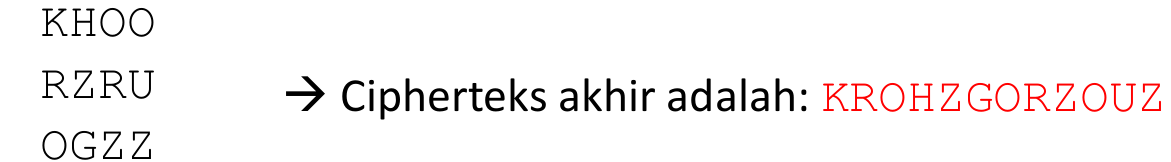
\includegraphics[width=128.10mm,height=44.55mm]{../../images/llm/page_041_img_01.png}%
\end{textblock*}

\end{document}
